\documentclass[12pt]{article}
\usepackage[dvips]{epsfig}
\usepackage{url}
\usepackage[colorlinks=true]{hyperref}

\begin{document}

\section*{GENESIS: Documentation}

{\bf Related Documentation:}
% start: userdocs-tag-replace-items related-do-nothing
% end: userdocs-tag-replace-items related-do-nothing

\section*{Create a New Document}

\subsection*{Introduction}

The GENESIS Documentation System is fully automated with versioning under the control of \href{http://monotone.ca/}{\bf monotone}. To learn more about monotone and its use by GENESIS see \href{../version-control/version-control.tex}{\bf Version\,Control} and to learn more about the levels of GENESIS documentation see \href{../documentation-overview/documentation-overview.tex}{\bf Documentation\,Overview}. This document assumes that you are familiar with that material.

Here, we introduce some of the flexibility, features, and requirements of the GENESIS Documentation System. We describe the location of source files within this system, the contents of a documentation folder/directory, and how to create a new document.

To learn how to add a new document to the GENESIS version control system see \href{../version-control/version-control.tex}{\bf Version\,Control}. Once a document is under version control and identified with the correct tags (see below) it can be automatically published from your local computer to the GENESIS website (\href{http://www.genesis-sim.org/}{www.genesis-sim.org}) to be available for other members of the GENESIS community.

\subsection*{Location of GENESIS Documentation}

Following a \href{../genesis-installation/genesis-installation.tex}{\bf Developer\,Installation} the documents that make up the GENESIS Documentation System are located in your local workspace. The default location of your local workspace is:
\begin{verbatim}
    ~/neurospaces_project/userdocs/source/snapshots/0
\end{verbatim}
The source materials for individual GENESIS documents are located in uniquely named folders/directories in your local workspace. One of the directories in the workspace is named\,{\it NewDocument}. This directory and the files it contains provide the templates for a generic GENESIS document. The files included by default are\,{\it descriptor.yml} and\,{\it NewDocument.tex}, and a sub-directory named\,{\it figures}.

\subsubsection*{The Default YAML Descriptor File}

The name of the descriptor file\,{\it descriptor.yml} should not be changed. The default contents of this file include: attributes (terminated by a colon) and tags (indicated by a hyphen), for example:

\begin{verbatim}
---
comment: Optional comment.
description: Briefly describe document contents here. 
document name: Insert a user readable document name here.
tags:
  - genesis3
  - level2
  - published
\end{verbatim}

\begin{itemize}

\item[]{\tt ---} The three dashes on the first line of the file {\it descriptor.yml} are part of the \href{http://yaml.org}{\bf YAML} syntax for automated software engineering. \\
{\bf Note:} The meaning of the white space/indents in the\,{\it descriptor.yml} file is defined for YAML.

\item[]{\tt comment:} Optional comment about the documentation file, e.g. reason for being tagged {\tt -\,obsolete}.

\item[]{\tt description:} The default file description ``Briefly describe file contents here.'' should be replaced with a short description of the subject matter of the documentation file. It is recommended that this file description is less than 80 characters on a single line.

\item[]{\tt document\,name:} Provide a document name which gives the title of the documentation file. This name is used as a link to the given file in the GENESIS Documentation System. This name is independent of and should be more human readable than the actual name of the document file it identifies.

\item[]{\tt tags:} List of tags used to identify the current document and locate it correctly in the documentation hierarchy. The default tags include {\tt -\,genesis3}, {\tt -\,level2}, and {\tt -\,published}. These tags indicate that the document is part of the GENESIS Documentation System at the level of User Guides and Documentation (Level 2) and that that the document will be published when documentation is rebuilt (see \href{../neurospaces-cron/neurospaces-cron.tex}{\it neurospaces\_cron}), but that in the absence of a {\tt - contents-level2} tag, the document name will not appear in the Level 2 Contents index (see below).

\begin{itemize}
   \item New tags may be created by adding them to the {\it descriptor.yml} file, but see below for a list of the tags currently recognized.  {\bf Note:} The tagging system is case insensitive to avoid tag duplication.

   \item Importantly, each of the directories {\tt contents-level1}\,\ldots {\tt contents-level7} in your local workspace contains a list of the documentation to be found at the given level. These content indices are generated automatically during a GENESIS installation, a {\tt userdocs} module installation, or a GENESIS update. They provide direct links to all documents tagged for the given level of documentation.
\end{itemize}   
\end{itemize}
Two important attributes are not included in the default {\it descriptor.yml} file, but may be added as required:
\begin{itemize}
\item[]{\tt redirect:} If present, this attribute is followed by a user supplied URL and automatically generates a HTTP redirect during a documentation system build. This allows documentation external to the GENESIS Documentation System to be automatically incorporated in the absence of any local documentation (with the exception of the {\it descriptor.yml} file). See \href{../http-redirect/http-redirect.tex}{\bf HTTP\,redirect} for an example.
\item[]{\tt summary:} If present, this attribute is followed by a short user supplied description of the contents of the document. This description will appear after the document name on the contents index page of the documentation level given by (for example here) the {\tt -\,contents-level2} tag.

\end{itemize}

\subsubsection*{The Default Documentation Source File}

Source files for the GENESIS Documentation System are currently produced with the \LaTeX\,typesetting package (see \href{http://www.latex-project.org/}{\bf www.latex-project.org}). It is planned that Microsoft Word ({\tt .doc} format) and OpenOffice ({\tt .odt}, ODF format) file formats will also be automatically recognized by the GENESIS Documentation System.

The default \LaTeX\, documentation source file\,{\it NewDocument.tex} in the {\it NewDocument} folder can be compiled to produce a readable PDF file. It gives help and examples for colorizing text, generating static hyperlinks to local and remote documentation, and how to insert a figure into your documentation.

\subsubsection*{The Figures Folder}

This directory contains any figures that your new document source file may include. The name of this folder should not be changed.
 
\section*{Create a New Document}

There are four simple steps to the creation of a new document within the GENESIS Documentation System.

\begin{enumerate}

\item[]{\bf Create document:}  To automatically create one or more new document template structures, simply envoke the {\it userdocs-create} script at a terminal command line prompt and give the name of the document you wish to create as an argument:
\begin{verbatim}
   userdocs-create <my-document>
\end{verbatim}
This command creates a new document folder/directory and its sub-directories by copying the template {\it NewDocument} file and assigning the given document name to both the documentation folder (here, for example, it would be {\it my-document}) and the default documentation file it contains (here, {\it my-document.tex}). It also inserts a description and a document name into the {\it descriptor.yml} file.

You can also specify multiple document names to create a series of documents:
\begin{verbatim}
   userdocs-create <my-document1> <my-document2> <my-document3> . . .
\end{verbatim}
{\bf Important:} It is a requirement of the GENESIS Documentation System that the names of the descriptor file\,{\it descriptor.yml} and the directory\,{\it figures} located in the document folder should not be changed.

For more details see \href{../document-create-manual/document-create-manual.tex}{\bf Manual\,Document\,Creation}. The remaining steps in document creation are currently manual.

\item[]{\bf Add Related Document Hyperlinks:} Hyperlinks to one or more related documents are by default located at the beginning of each document source {\tt .tex} file following the {\bf Related Documentation} heading. There are two ways to add links here:
\begin{itemize}
\item[] {\bf Hyperlinks to Manually Created GENESIS Documentation:} For Level\, 1 and 2 documentation, this is done in the usual way with the \LaTeX\, {\it href} command. See \href{../NewDocument/NewDocument.tex}{\bf New\,Document} for an implementation example .

\item[] {\bf Hyperlinks to Automatically Generated GENESIS Documentation:} Hyperlinks to the automatically generated documentation of Levels\,3--7 requires a tagging construct. This is by default located at the beginning of each document source {\tt .tex} file following the {\bf Related Documentation} heading. The generation of these links is controlled by a tagging construct which is automatically expanded whenever the document system is rebuilt:
\begin{verbatim}
   % start: userdocs-tag-replace-items <related-do-nothing>
   % end: userdocs-tag-replace-items <related-do-nothing>
\end{verbatim}

The default tag for this system is {\tt <related-do-nothing>}, which allows a document to be created and published in the absence of any related hyperlinks. 

More than one related document hyperlink can be added to a document by the addition of tags you create that replace the default tag. For example:
\begin{verbatim}
   % start: userdocs-tag-replace-items <your-tag-name1> <your-tag-name2> <your-tag-name3> . . .
   % end: userdocs-tag-replace-items <your-tag-name1> <your-tag-name2> <your-tag-name3> . . .
\end{verbatim}

As shown in the above example, the related tag(s) should have the following form:
\begin{verbatim}
   related-<your-tag-name1>
\end{verbatim}
where {\tt <your-tag-name1>} is replaced by an identifier you create. % Importantly, this tag must also be placed in the {\it descriptor.yml} file of the document you want the hyperlink to reference.

{\bf Note:} The default related document hyperlink {\tt related-do-nothing} relies on a document called \href{../do-nothing/do-nothing.tex}{\it do-nothing.tex}.
\end{itemize}

\item[]{\bf Update the descriptor.yml file:} Each directory/file in the GENESIS Documentation System is tagged on the basis of its content, for example:

   \begin{enumerate}

      \item[]{\bf The GENESIS version:} This tags the version of GENESIS that the document refers to, e.g. {\tt -\,genesis3}.

      \item[]{\bf Level of the GENESIS document:} This must be one of the seven levels of the GENESIS Documentation System, which include:
      
      \begin{itemize}
         \item[]\href{../contents-level1/contents-level1.tex}{\tt -\,level1} (introductory documentation)
         \item[]\href{../contents-level2/contents-level2.tex}{\tt -\,level2} (user/developer documentation)
         \item[]\href{../contents-level3/contents-level3.tex}{\tt -\,level3} (autogenerated documentation)
         \item[]\href{../contents-level4/contents-level4.tex}{\tt -\,level4} (autogenerated technical documentation)
         \item[]\href{../contents-level5/contents-level5.tex}{\tt -\,level5} (autogenerated algorithm documentation)
         \item[]\href{../contents-level6/contents-level6.tex}{\tt -\,level6} (autogenerated api documentation)
         \item[]\href{../contents-level7/contents-level7.tex}{\tt -\,level7} (inline source code documentation)
      \end{itemize}
{\bf Important:} When creating a new document, the default tag ({\tt -\,level2}) in the associated {\it descriptor.yml} file should be replaced with a tag from the above list that identifies the correct level of the document.

For more on the levels of the GENESIS Documentation System see the \href{../documentation-overview/documentation-overview.tex}{Documentation\,Overview}.

\item[]{\bf Tag Appearance of Document Name in Contents Index:} A document name (given by the {\tt document\,name:} attribute) will not appear in the documentation contents list unless one of the {\tt -\,contents-level1}$\ldots${\tt -\,contents-level7} tags is present in the associated {\it descriptor.yml} file. The presence of this tag results in the document name being placed in alphabetical order in the contents page of the level specified by the tag. If you do not want the name of the document to appear in the contents page you should remove this tag. This functionality allows one or more documents to be hyperlinked from a summary document (see particularly Level 1 and 2 documentation) without the name of the hyperlinked document(s) also appearing in the contents page of the given level.

\item[]{\bf Insert ``Related Document'' hyperlink tags:} To link a new document (Referring Document in following figure) to another document (Referenced Document in following figure) under its {\bf Related Documentation} section, place the appropriate tag after the tag construct at the head of the Referring Document and place the same tag in the {\bf descriptor.yml} file of the Referenced Document. The following figure illustrates these relationships.
\begin{figure}[h]
  \centering
   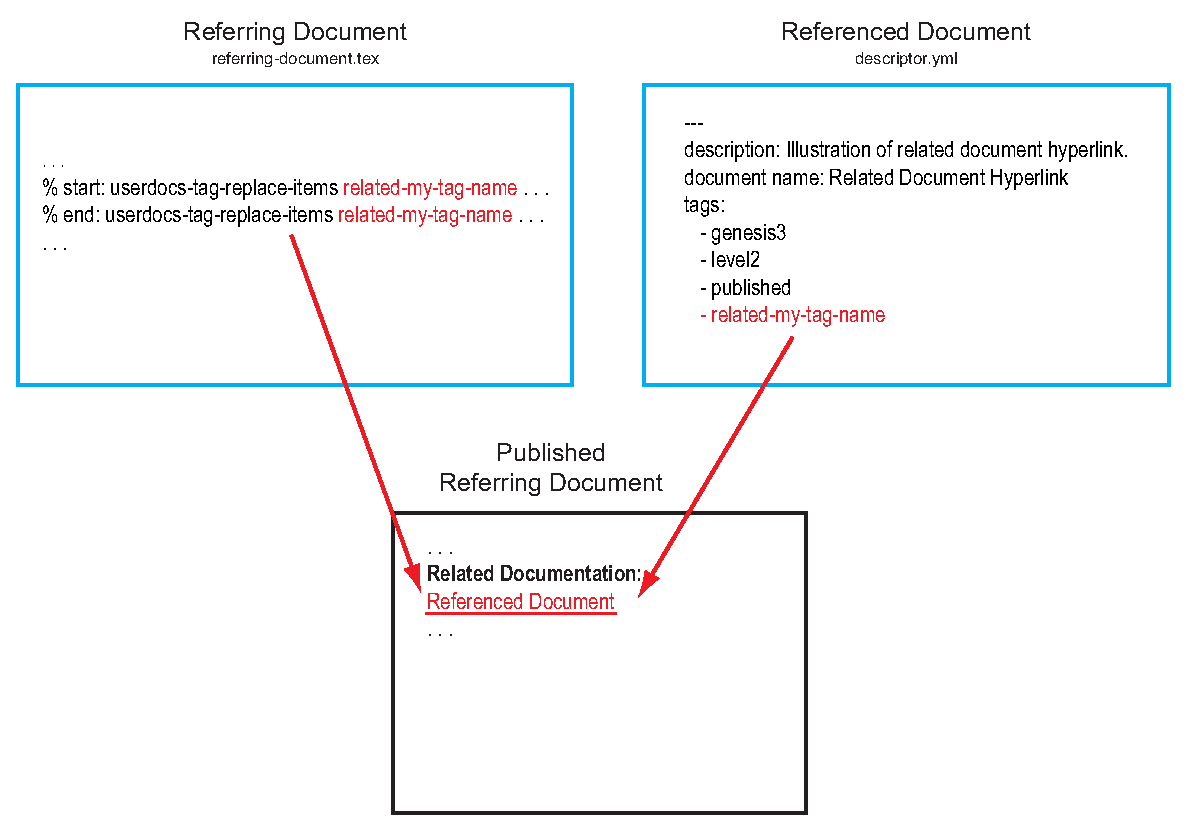
\includegraphics[scale=0.8]{figures/related-document.eps}
%\caption{{\bf A Dummy Figure:} Example of \LaTeX\,\,\,code to incorporate a figure into documentation.}
%  \label{fig:df-2}
\end{figure}

\item[]{\bf Tag document origin:} If the document has been created from one located on the \href{http://code.google.com/p/neurospaces/w/list}{\bf Neurospaces\,wiki} then a {\tt --wiki} tag should be inserted in the {\it descriptor.yml} file.

\item[]{\bf Tag document status:} For a given document to be part of the documentation version control system and the GENESIS Documentation System, it must be in a documentation folder along with a {\it descriptor.yml} file that contains only one of either the {\tt -\,draft}, {\tt -\,local}, or {\tt -\,published} tags. {\bf Note:} The {\tt-\,published} tag in the {\it descriptor.yml} file associated with your new document should be replaced with the {\tt -\,draft} tag  while you are working on the document to prevent it being published to the GENESIS website. 

{\bf Precedence of publication related tags:} Three tags control publication of documents within the GENESIS Documentation System. They are interpreted in a hierarchical manner, such that the presence of the {\tt  -\,draft} tag along with either the {\tt -\,local} and/or {\tt -\,published} tag will prevent the document from being included into a build/update of the Documentation System. Alternatively, a document will not be published to be browser viewable in the absence of either the {\tt -\,local} or {\tt -\,published} tag. So if documentation is (not) appearing where you expect after an update, it is a good idea to check the publication tags in the {\it descriptor.yml} file.

\begin{itemize}
	\item[]{\tt -\,draft}: The presence of this tag in the\,{\it descriptor.yml} file associated with a document will prevent the document 
	from being published,  i.e. viewable within a browser. For a document to be publishable, the {\tt -\,draft} tag must be replaced 
	with either the {\tt -\,local} or the {\tt -\,published} tag.
	
	\item[]{\tt -\,local}: This tag indicates that a document will be included into any local build of the the GENESIS Documentation 
	System. The presence of this tag means that a document will be browser viewable on (a) local machine(s), but will not appear as a 
	`published' document on the GENESIS web site at {\tt http://genesis-sim.org}. This tag is useful to developers for checking documentation
	prior to publication on the web via the GENESIS web site and can be used to control who can view documentation locally.
	
	\item[]{\tt -\,published:} The presence of this tag in the\,{\it descriptor.yml} file will cause the associated document to be published to the 
	GENESIS Documentation System on the GENESIS web site, as long as neither the {\tt -\,draft} nor the {\tt -\,local} tags are present in the same
	\,{\it descriptor.yml} file (see next item). Similarly, absence of the {\tt -\,draft} tag but presence of the {\tt -\,local} tag will prevent publication of a 
	document to the GENESIS web site even if the {\tt -\,published} tag is present.

\end{itemize}

Tags in the descriptor file currently recognized by the documentation build system include:
\begin{verbatim}
  tags:
    - contents-level1
    - contents-level2
    - contents-level3
    - contents-level4
    - contents-level5
    - contents-level6
    - contents-level7
    - draft
    - local
    - published
    - obsolete
    - html
    - pdf
    - png
    - ps
    - mp3
    - wav    
\end{verbatim}

Other useful tags include:
\begin{verbatim}
    - genesis2
    - genesis3
    - level1
    - level2
    - level3
    - level4
    - level5
    - level6
    - level7
    - wiki
    - create
    - introduction
    - tutorial
    - document
\end{verbatim}

{\bf Note:} User supplied tags not recognized by the documentation build system may still be useful for local control and sorting of documentation. Importantly, when adding your own tags remember that the interpretation of the\,{\it descriptor.yml} file by the GENESIS Documentation System is sensitive to white space and indents.
 
\end{enumerate}

\item[]{\bf Update the\,{\it figures} folder:} Place any figures or images, etc that your source document file contains in the\,{\it figures} directory.

\end{enumerate}

\subsection*{Incorporate References in Your Document}

The GENESIS Documentation System currently supports \href{http://www.bibtex.org/}{\bf BibTeX} by default. The two \LaTeX commands at the end of the {\it NewDocument} template enable this functionality. They are:
\begin{verbatim}
   \bibliographystyle{plain}
   \bibliography{../tex/bib/g3-refs.bib}
\end{verbatim}
These commands allow you to define a citation style for your references and give the location of a file that complies with the BibTex file format requirements and contains your bibliography. Currently, the default name of this file is {\it g3-refs.bib}. It contains all the references for the \href{../publication/publication.tex}{\bf GENESIS Publication System}.

\subsection*{Incorporate a Pre-existing Document, File, or Video}

The GENESIS Documentation System recognizes a number of different file formats. The purpose is to allow preexisting documentation to be directly included without having first to be converted to the \LaTeX\,format.

To incorporate a pre-existing document into the GENESIS Documentation System:

\begin{enumerate}

\item Include a tag in the {\it descriptor.yml} file in the document directory. Currently, the following file format tags are recognized (Note. No tag is necessary for either \LaTeX\,files as the {\tt .tex} file name suffix is the default for the GENESIS Documentation System or {\tt .eps} files in the {\it figures} folder):

\begin{itemize}

\item[]{\bf - eps} Encapsulated postscript.
%\item[]{\bf - html} Hypertext markup language.
\item[]{\bf - pdf} Portable document format.
%\item[]{\bf - png} Portable network graphics.
%\item[]{\bf - ps} Postscript.

\end{itemize}

\item Place the document file in the document directory (NOT the {\it figures} sub-directory).

\end{enumerate}

It is also possible to incorporate audio and video files as part of documentation. Currently recognized audio file format tags include:

\begin{itemize}
   \item[]{\bf - wav} Microsoft .wav file format.
   \item[]{\bf - mp3} Digital audio encoding format.
\end{itemize}

To incorporate video into a GENESIS document: 

\begin{enumerate}
   \item Create an account with a video sharing website, e.g. \href{http://www.youtube.com/watch?v=1n8DxTk2gVM}{\bf YouTube}.
   \item Upload your video(s).
   \item Embed a link to the video(s) into the document describing their contents. See \href{../NewDocument/NewDocument.tex}{\bf NewDocument}, for further details.
\end{enumerate}

{\bf Note:} With document incorporation (c.f. creation) the document to be included is located in the {\it $<$document-name$>$} directory and NOT the {\it figures} subdirectory.

\subsection*{Document Version Tracking and Control}

To learn more about document version tracking and control in the GENESIS Documentation System, see \href{../version-control/version-control.tex}{\bf Version\,Control}.

\subsection*{Document Hyperlink Checking}

The validity of the hyperlinks embedded in GENESIS documentation (see \href{../NewDocument/NewDocument.tex}{\bf NewDocument}) are checked by {\it userdocs\_cron} each time the GENESIS Documentation System is rebuilt. The output of this check can be viewed at \href{http://www.genesis-sim.org/userdocs/webcheck/badlinks.html}{\bf www.genesis-sim.org/userdocs/webcheck/badlinks.html}.

Webcheck can also be run locally to check hyperlinks. When run in the
\begin{verbatim}
   ~/neurospaces_project/userdocs/source/snapshots/0
\end{verbatim}
directory, the command {\tt make\,webcheck} will produce a report in
\begin{verbatim}
   ~/neurospaces_project/userdocs/source/snapshots/0/html/htdocs/neurospaces_project/userdocs/webcheck/
\end{verbatim}

\subsection*{Document Publication}

To learn more about the automated publication of documents in the GENESIS Documentation System, see \href{../publication/publication.tex}{\bf Publication}.


\end{document}
